\documentclass{article}
\usepackage{amssymb}
\usepackage{babel}
\usepackage{geometry}
\usepackage{amsmath}
\usepackage{amsthm}
\usepackage{framed}
\usepackage{pifont}
\usepackage{listings}
\usepackage{graphicx}
\usepackage{subcaption} 
\usepackage{subcaption} 
\usepackage{booktabs}
\usepackage{multirow}
\usepackage{xcolor}
\usepackage{array}

\definecolor{codegray}{gray}{0.9}
\lstset{
    backgroundcolor=\color{codegray},
    basicstyle=\ttfamily\small,
    breaklines=true,
    frame=single
}


\def\ra{\rightarrow}
\def\oo{\infty}
\def\l/{\backslash}
\def\0{\emptyset}
\def\b{\,\,\,}
\def\mm{{\mu^*}}
\def\hm{\mathcal{H}^s}
\def\vm{\nu^*}
\def\cui{\bigcup_{i=1}^\infty}
\def\cai{\bigcap_{i=1}^\infty}
\def\cuj{\bigcup_{j=1}^\infty}
\def\caj{\bigcap_{j=1}^\infty}
\def\sumj{\sum_{j=1}^\infty}
\def\sumi{\sum_{i=1}^\infty}
\def\sumn{\sum_{n=1}^\infty}
\def\px{\mathcal{P}_X}
\def\s{\mathcal{S}}
\def\a{\mathcal{A}}
\def\bs{\mathcal{B}}
\def\lm{\mathcal{L}}
\def\R{\mathbb{R}}
\def\E{\mathbb{E}}
\def\Z{\mathbb{Z}}
\def\m{\mathcal{M}}
\def\rr{\Rightarrow}
\def\tf{$\Rightarrow$}
\def\f{\mathcal{F}}
\def\limn{\lim_{n \rightarrow \infty}}
\def\st{\text{s.t.}}
\def\sums{ \sum_{x \in \s}}

%Ricky Def
\def\baru{\bar{\mu}}
\def\Mbaru{\mathfrak{M}_{\baru}}


\title{COMP4211 PA2 Report} 
\author{Name: Ruiming Min; SID: 20827430; ITSC: rmin}
\date{\today}

\begin{document}

    
\maketitle

\section*{5 Datasets and Data Loaders}

\subsection*{5.3 Dataloader Implementation}

\subsubsection*{[Q1]}
Number of images in COCO dataset: 3557.
Number of images in WikiArt dataset: 7492.

\subsubsection*{[Q2]}
Number of images in PACS train dataset: 1641.
Number of images in PACS test dataset: 2723.

\section*{6 Style Transfer}

\subsection*{6.2 Model}

\subsubsection*{[Q3]}
Since after encoding, the image is represented as a 3D tensor and its 2D shape is much smaller than the original image. 
Therefore, in the decoder, we need the upsampling to re-construct the image to its original size.

\subsubsection*{[Q4]}
For eact layer, we have the trainable parameters as follows:
\begin{itemize}
    \item Conv2d: $(k \times k \times c_{in} + 1) \times c_{out}$
    \item Pooling and Upsampling: 0
\end{itemize}

Therefore, the total number of trainable parameters is 2332511.

\subsubsection*{[Q5]}
Since the we need encoder to encode the image and mine the features, but if we only use the encoder, we cannot re-construct the image. 
Therefore, we need the decoder to re-construct the image.

\subsubsection*{[Q6]}
Since in this model, we do not only need the style match our target style, but also need the content to be preserved.
Therefore, we need to use the content loss and style loss to balance the style transfer.

\subsubsection*{[Q7]}

After 55 epochs, total loss is 13021.544, content loss is 8052.103, and style loss is 4969.441.

\subsubsection*{[Q8]}

From the figure \ref{fig:part1_inference}, we can see the style transfer examples.
In these comparisons, we can see that the generated images represented the content of the content images very well expect the words in them.
For the style, the generated images are very similar to the style images in color and painting techniques.
However, if the style is very different from the content, the generated images may not be very good (e.g.: picture l).
Moreover, the generated images have some strange textures in some areas, which may be caused by the imbalance of the style data set, i.e., there are too many paintings in the training set.

% input images in a 3*2 grid
\begin{figure}[ht]
    \centering
    % First row of subfigures
    \begin{minipage}{\textwidth}
        \centering
        \begin{subfigure}{0.25\textwidth}
            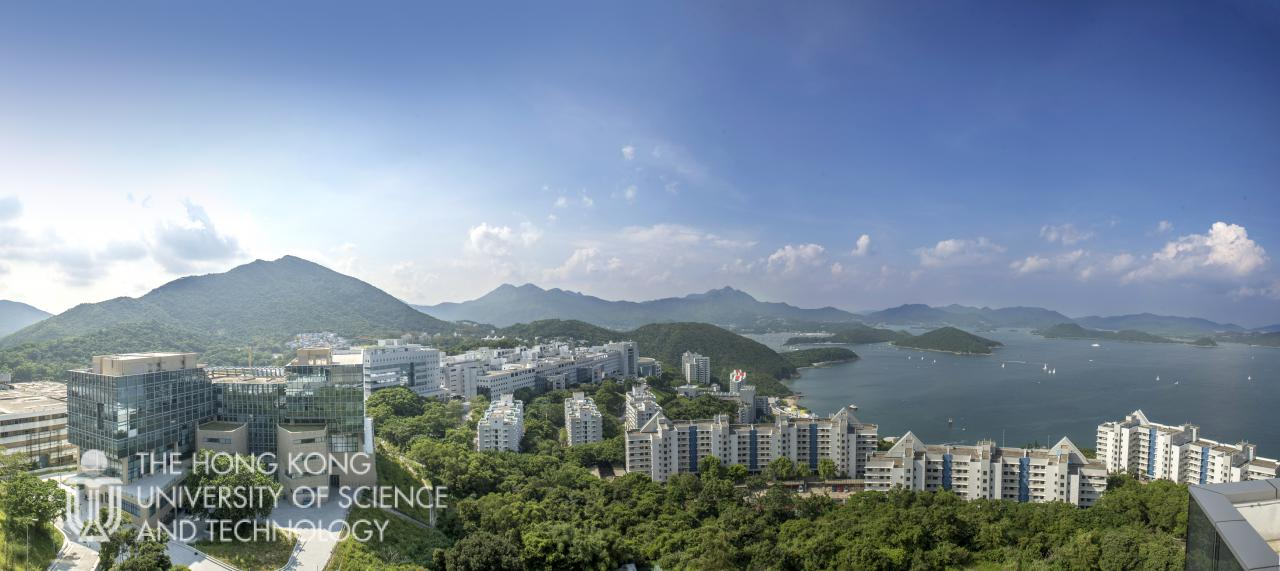
\includegraphics[width=\textwidth]{./data_set/HKUST/1.jpg}
            \caption{Content Image}
        \end{subfigure}
        \hfill % This command adds space between the subfigures
        \begin{subfigure}{0.25\textwidth}
            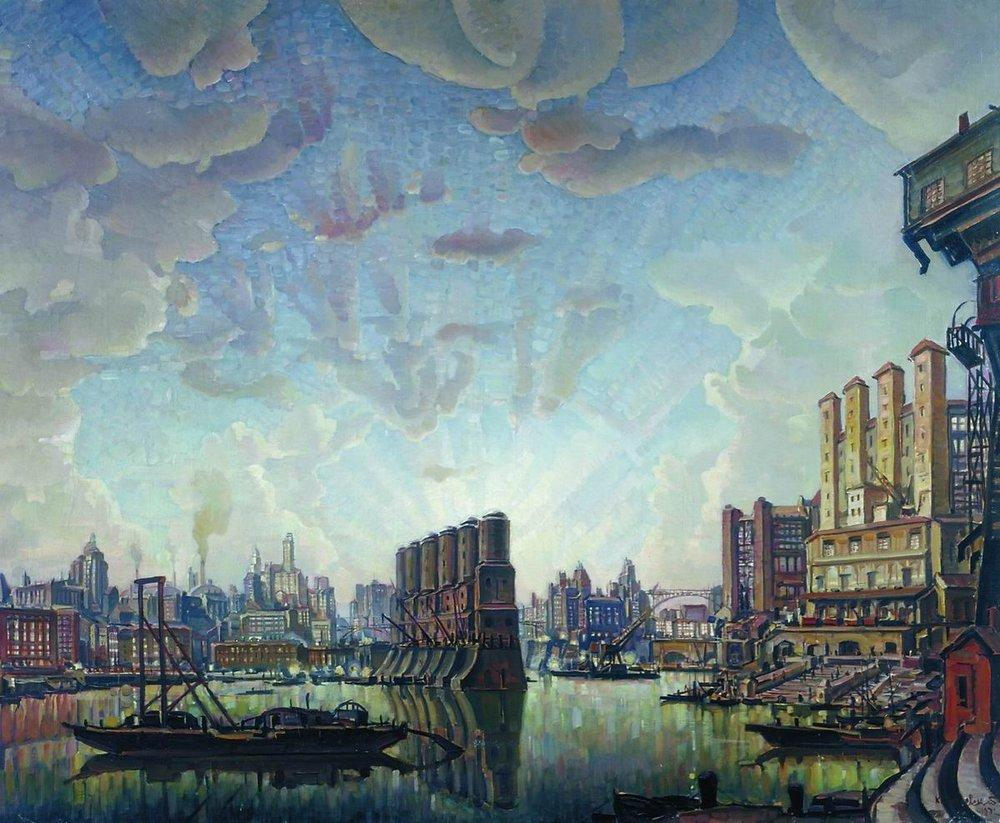
\includegraphics[width=\textwidth]{./wikiart/Symbolism/konstantin-bogaevsky_port-of-imaginary-city-1932.jpg}
            \caption{Style Image}
        \end{subfigure}
        \hfill % This command adds space between the subfigures
        \begin{subfigure}{0.25\textwidth}
            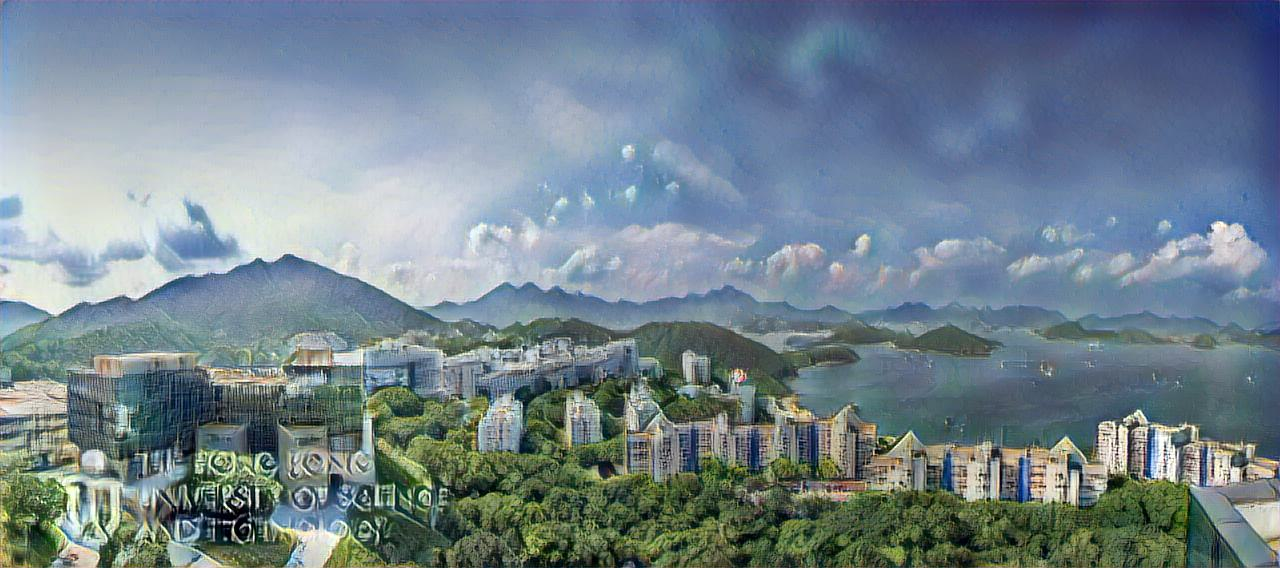
\includegraphics[width=\textwidth]{./part1_inference/output_1_konstantin-bogaevsky_port-of-imaginary-city-1932.jpg}
            \caption{Generated Image}
        \end{subfigure}
    \end{minipage}
    
    \vspace{0.1cm} % This command adds vertical space between the rows
    
    % Second row of subfigures
    \begin{minipage}{\textwidth}
        \centering
        \begin{subfigure}{0.25\textwidth}
            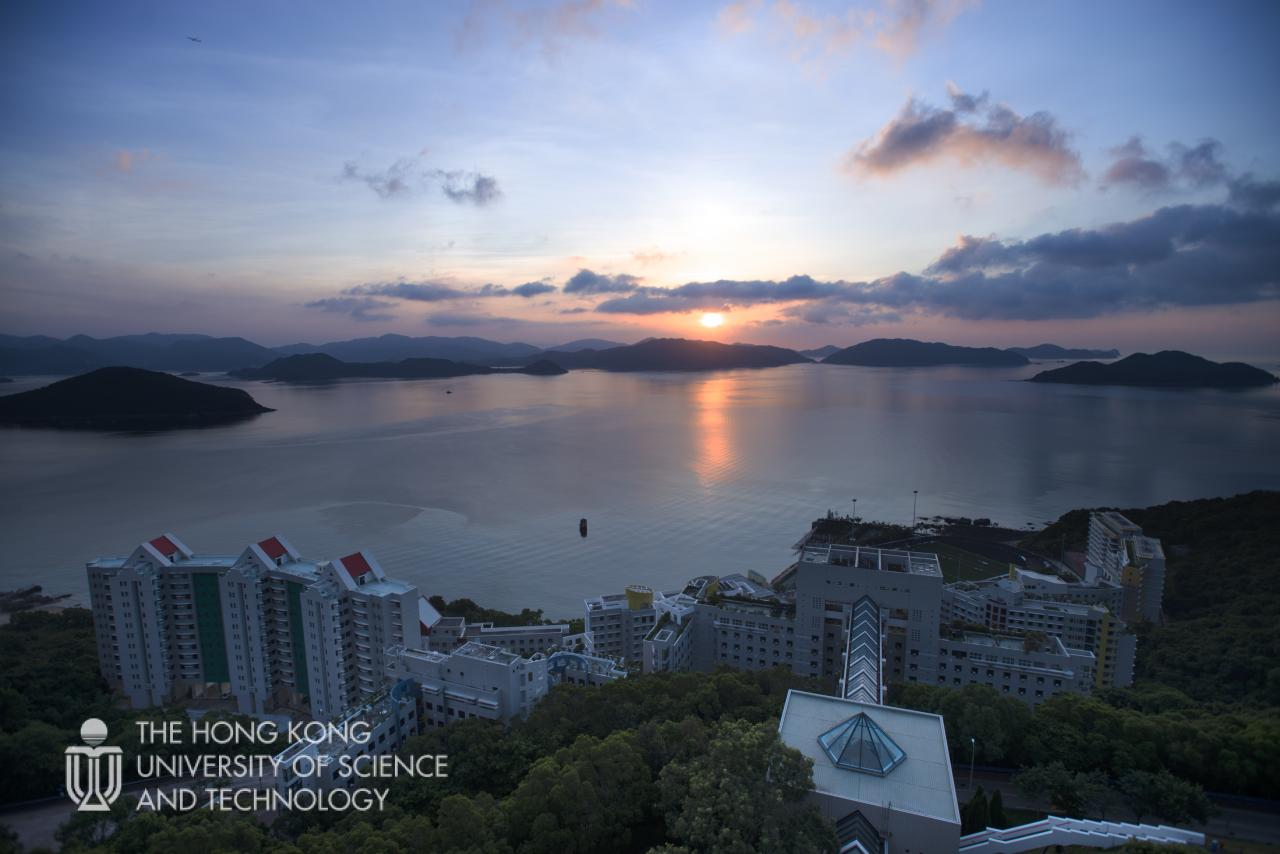
\includegraphics[width=\textwidth]{./data_set/HKUST/2.jpg}
            \caption{Content Image}
        \end{subfigure}
        \hfill % This command adds space between the subfigures
        \begin{subfigure}{0.25\textwidth}
            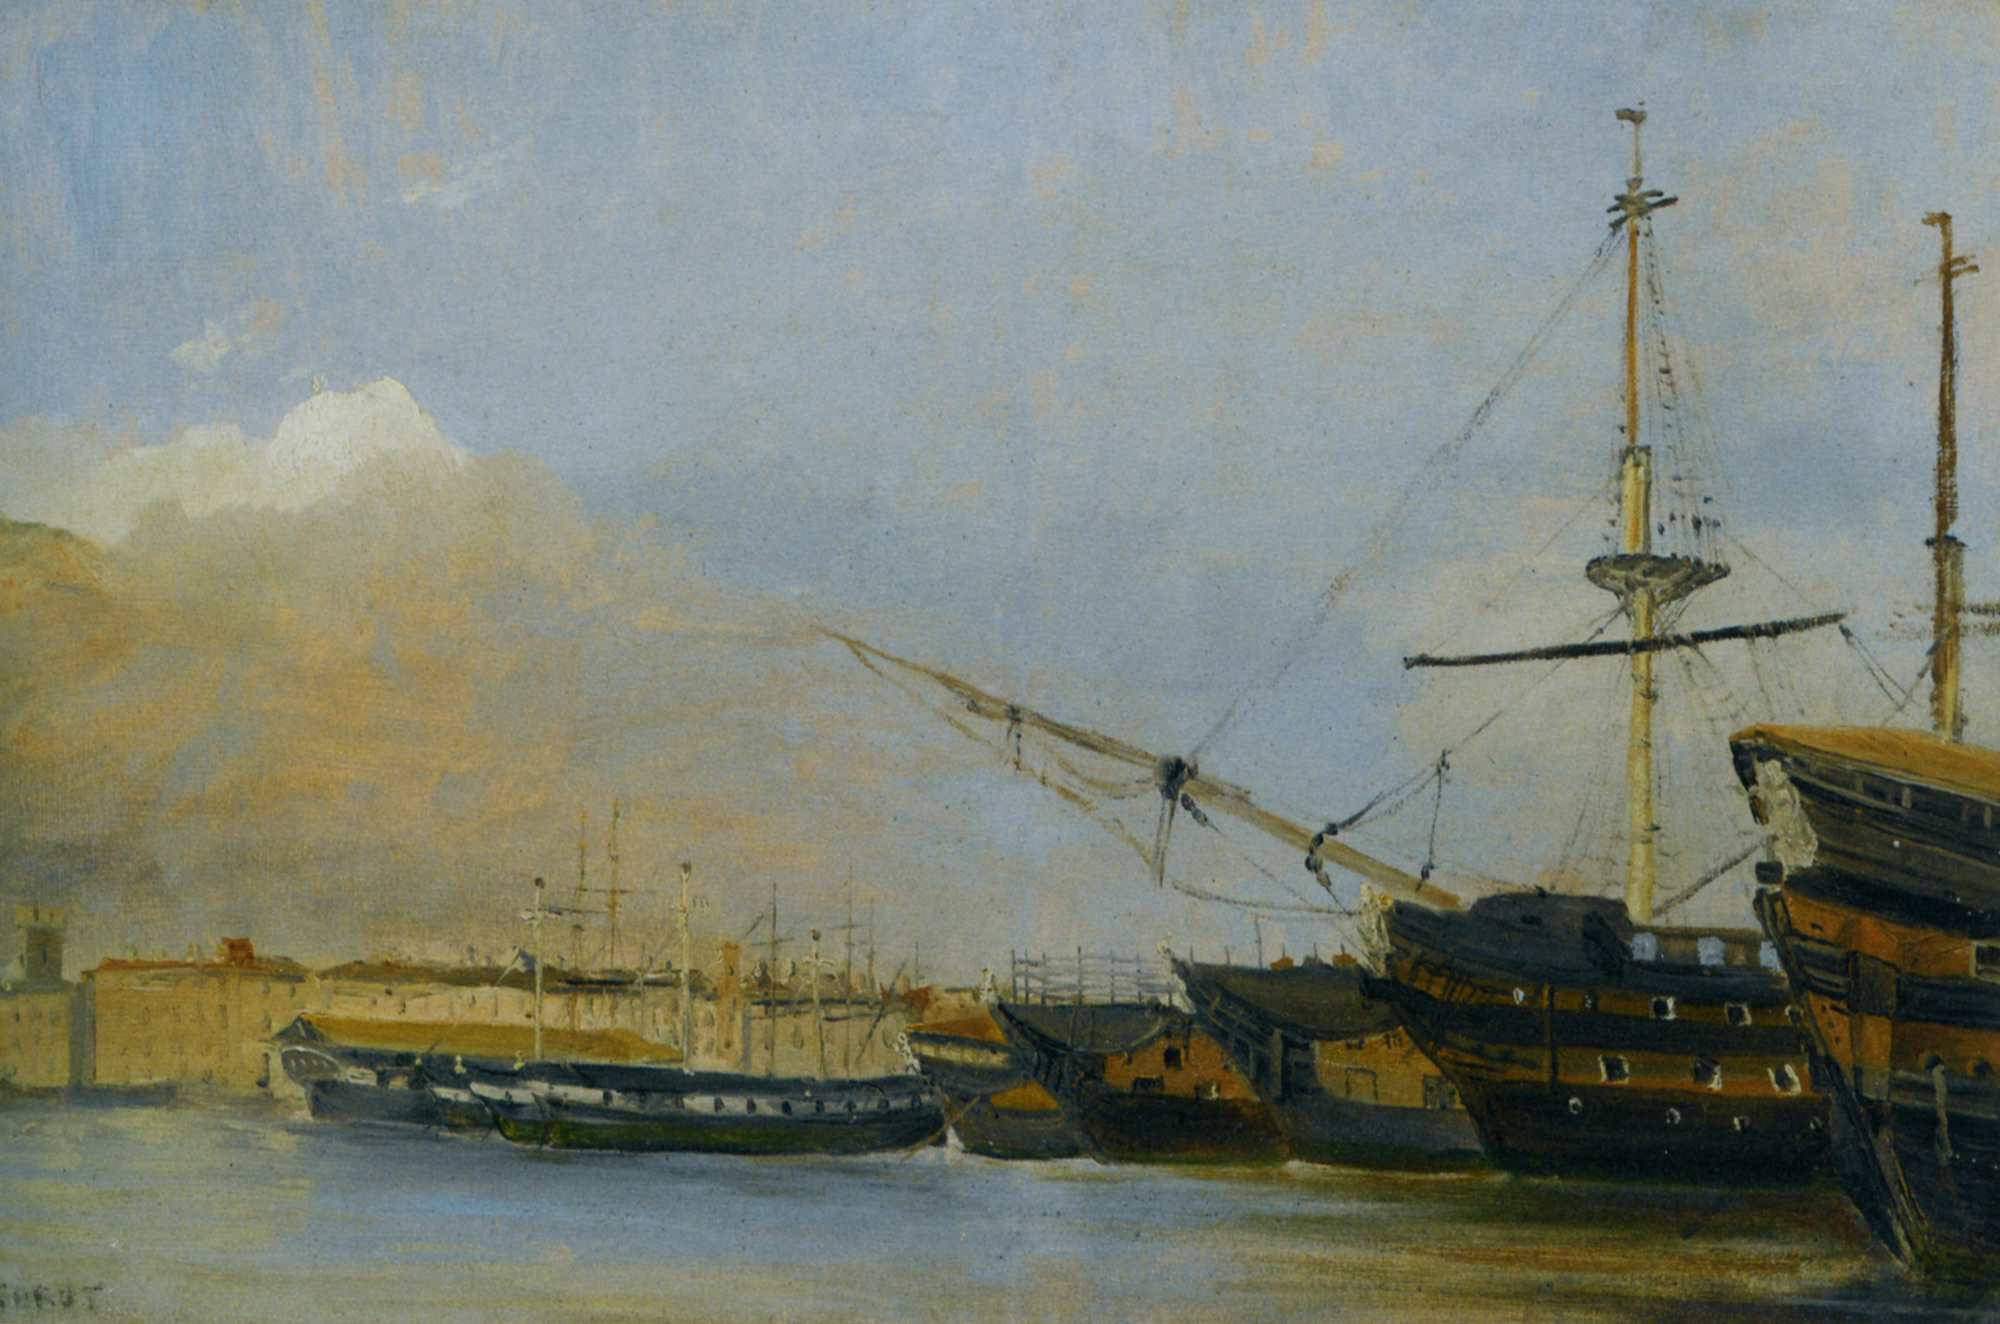
\includegraphics[width=\textwidth]{./wikiart/Realism/camille-corot_toulon-battleships-dismantled.jpg}
            \caption{Style Image}
        \end{subfigure}
        \hfill % This command adds space between the subfigures
        \begin{subfigure}{0.25\textwidth}
            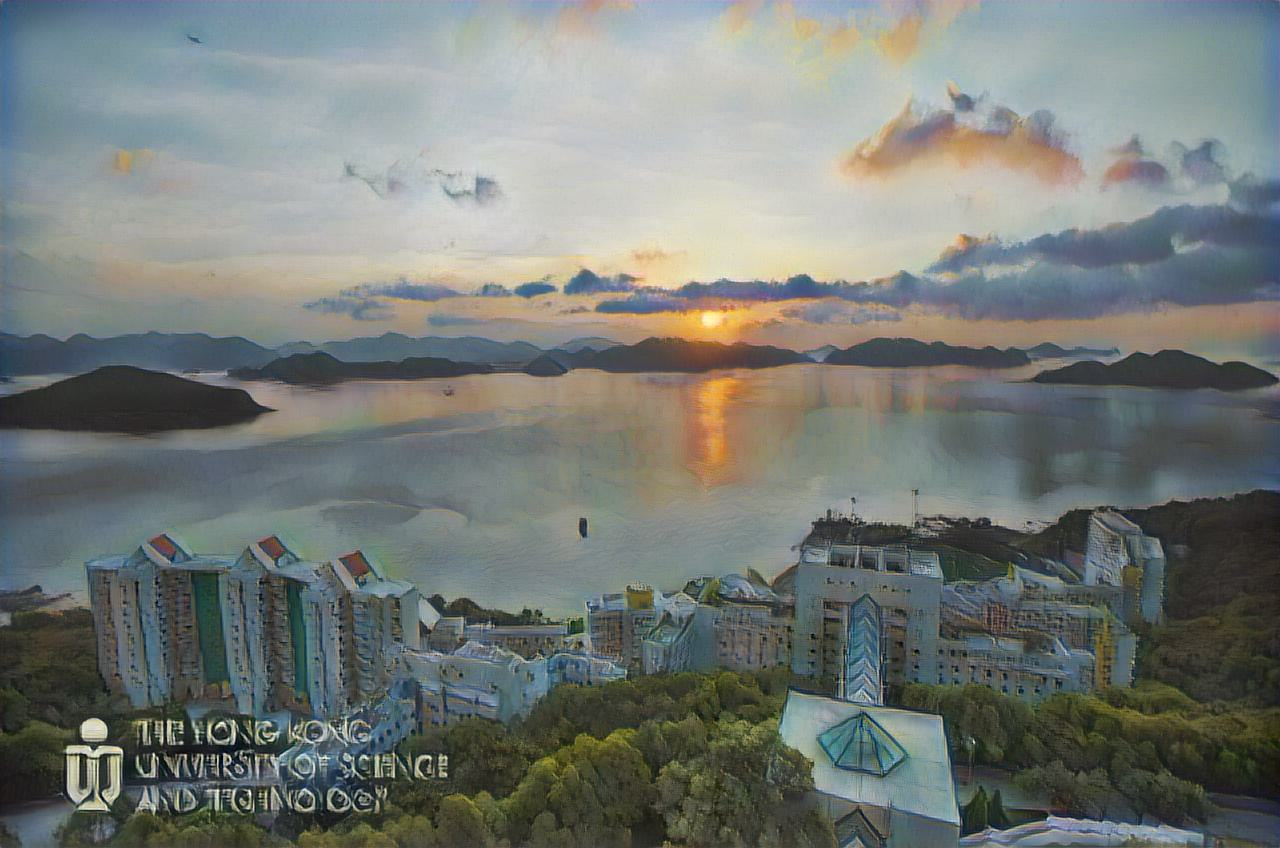
\includegraphics[width=\textwidth]{./part1_inference/output_2_camille-corot_toulon-battleships-dismantled.jpg}
            \caption{Generated Image}
        \end{subfigure}
    \end{minipage}
    
    \vspace{0.1cm}

    \begin{minipage}{\textwidth}
        \centering
        \begin{subfigure}{0.25\textwidth}
            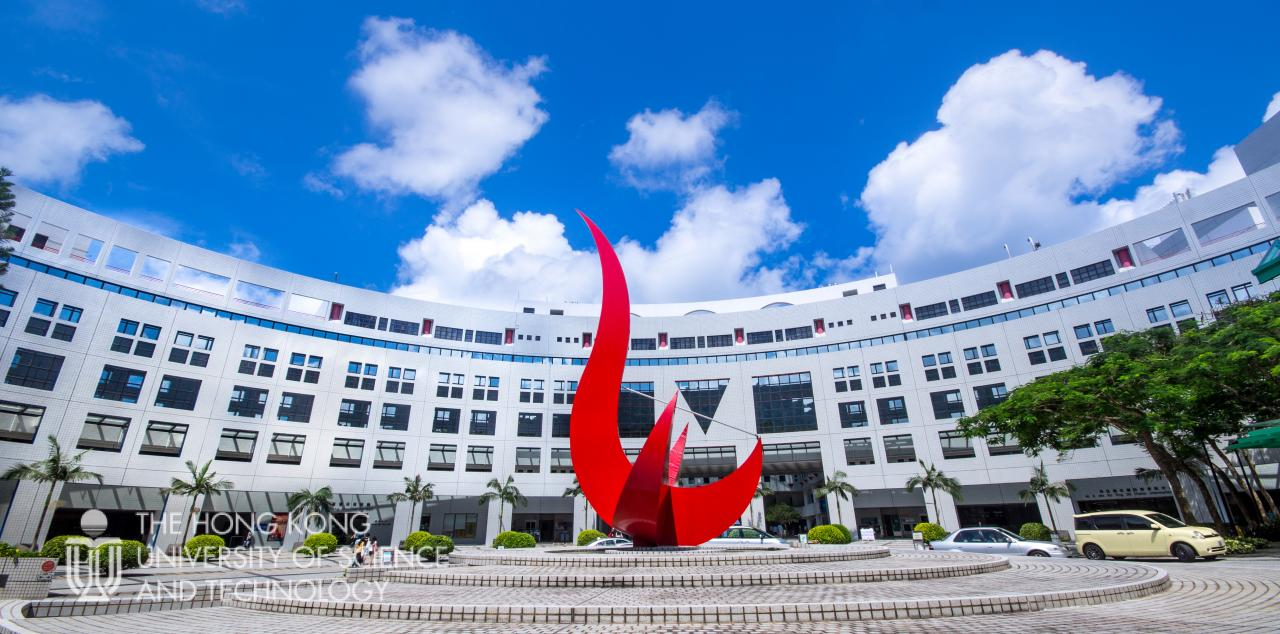
\includegraphics[width=\textwidth]{./data_set/HKUST/3.jpg}
            \caption{Content Image}
        \end{subfigure}
        \hfill % This command adds space between the subfigures
        \begin{subfigure}{0.25\textwidth}
            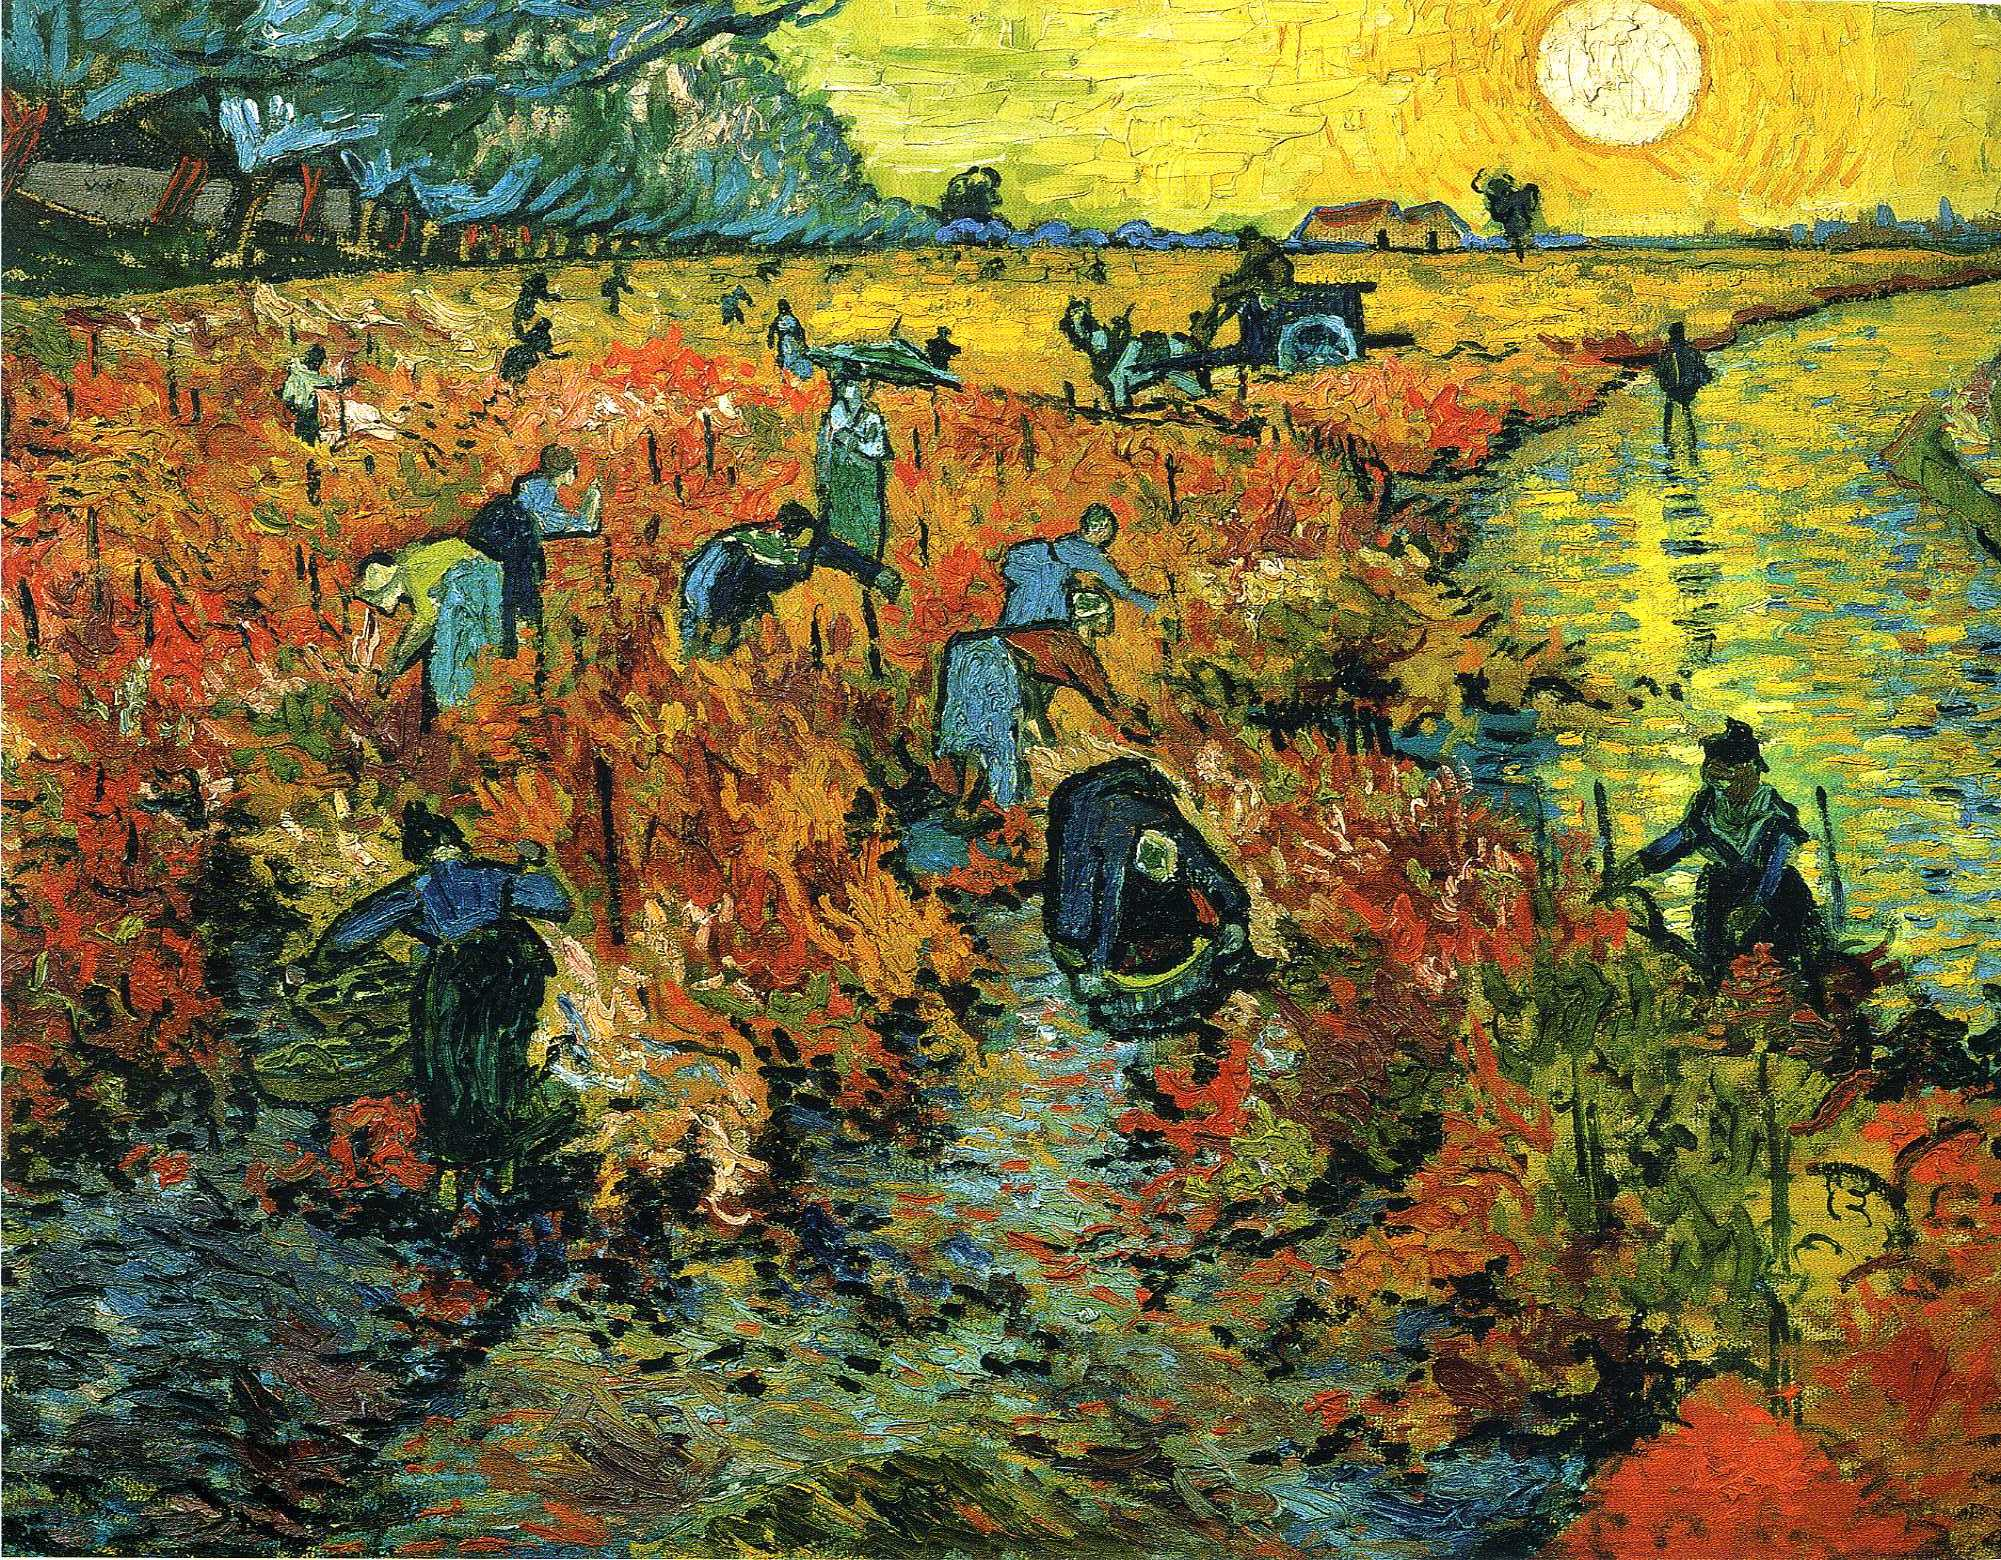
\includegraphics[width=\textwidth]{./wikiart/Post_Impressionism/vincent-van-gogh_red-vineyards-at-arles-1888.jpg}
            \caption{Style Image}
        \end{subfigure}
        \hfill % This command adds space between the subfigures
        \begin{subfigure}{0.25\textwidth}
            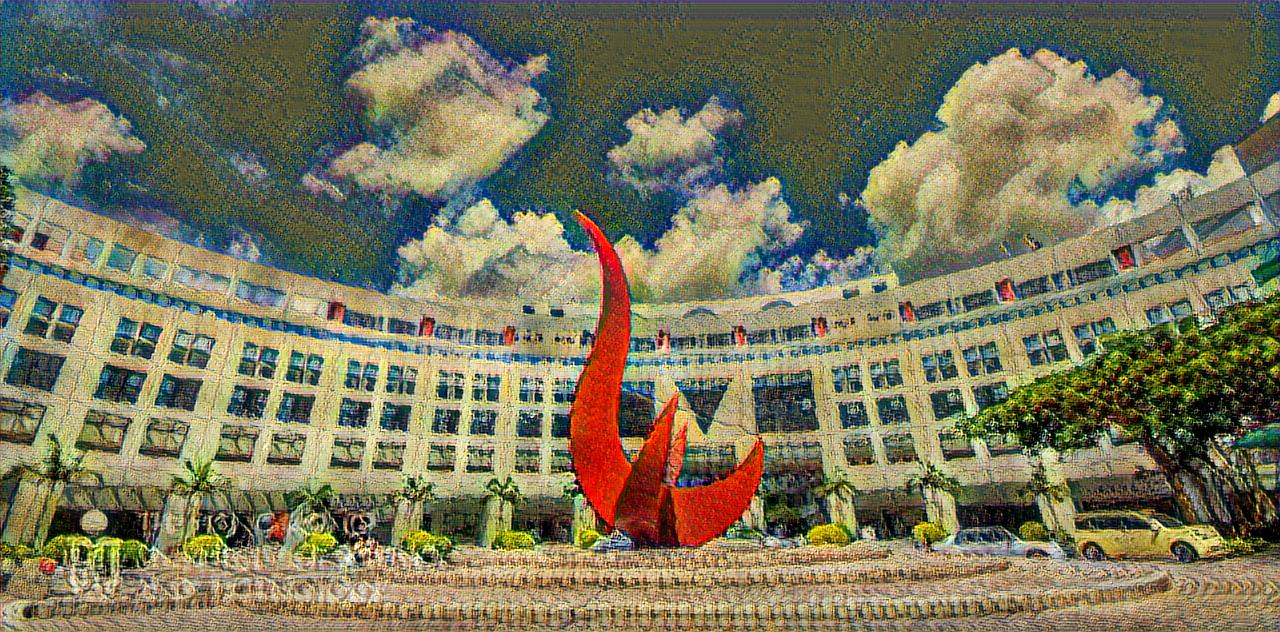
\includegraphics[width=\textwidth]{./part1_inference/output_3_vincent-van-gogh_red-vineyards-at-arles-1888.jpg}
            \caption{Generated Image}
        \end{subfigure}
    \end{minipage}
    
    \vspace{0.1cm}

    \begin{minipage}{\textwidth}
        \centering
        \begin{subfigure}{0.25\textwidth}
            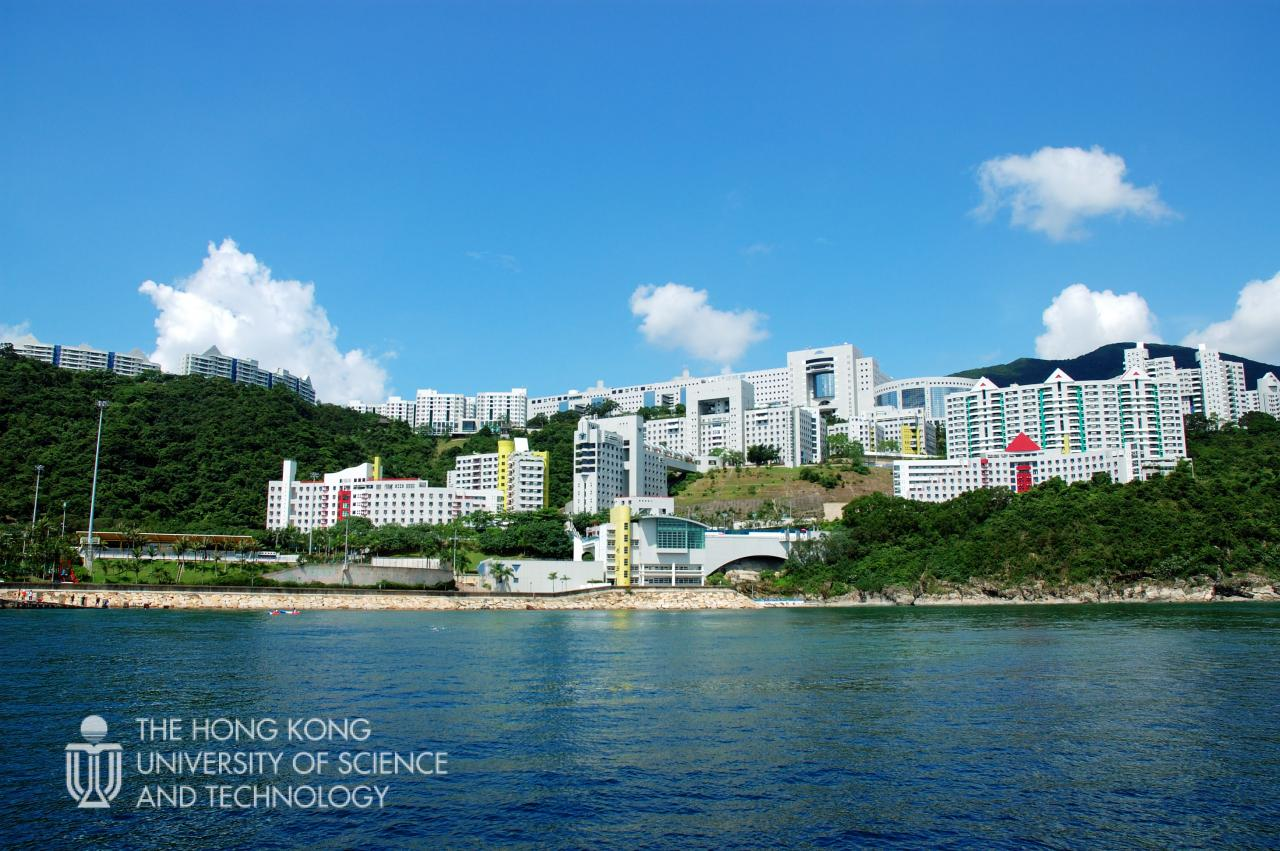
\includegraphics[width=\textwidth]{./data_set/HKUST/6.jpeg}
            \caption{Content Image}
        \end{subfigure}
        \hfill % This command adds space between the subfigures
        \begin{subfigure}{0.25\textwidth}
            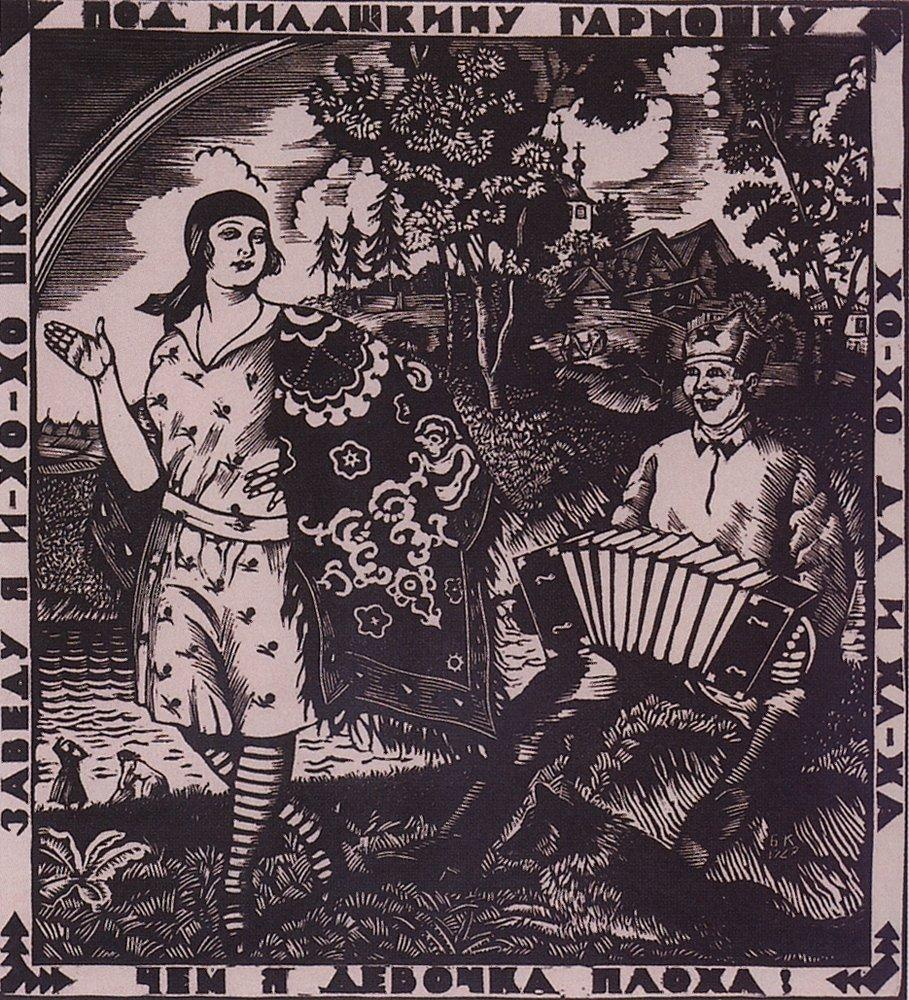
\includegraphics[width=\textwidth]{./wikiart/Art_Nouveau_Modern/boris-kustodiev_under-honey-s-harmonica-1927.jpg}
            \caption{Style Image}
        \end{subfigure}
        \hfill % This command adds space between the subfigures
        \begin{subfigure}{0.25\textwidth}
            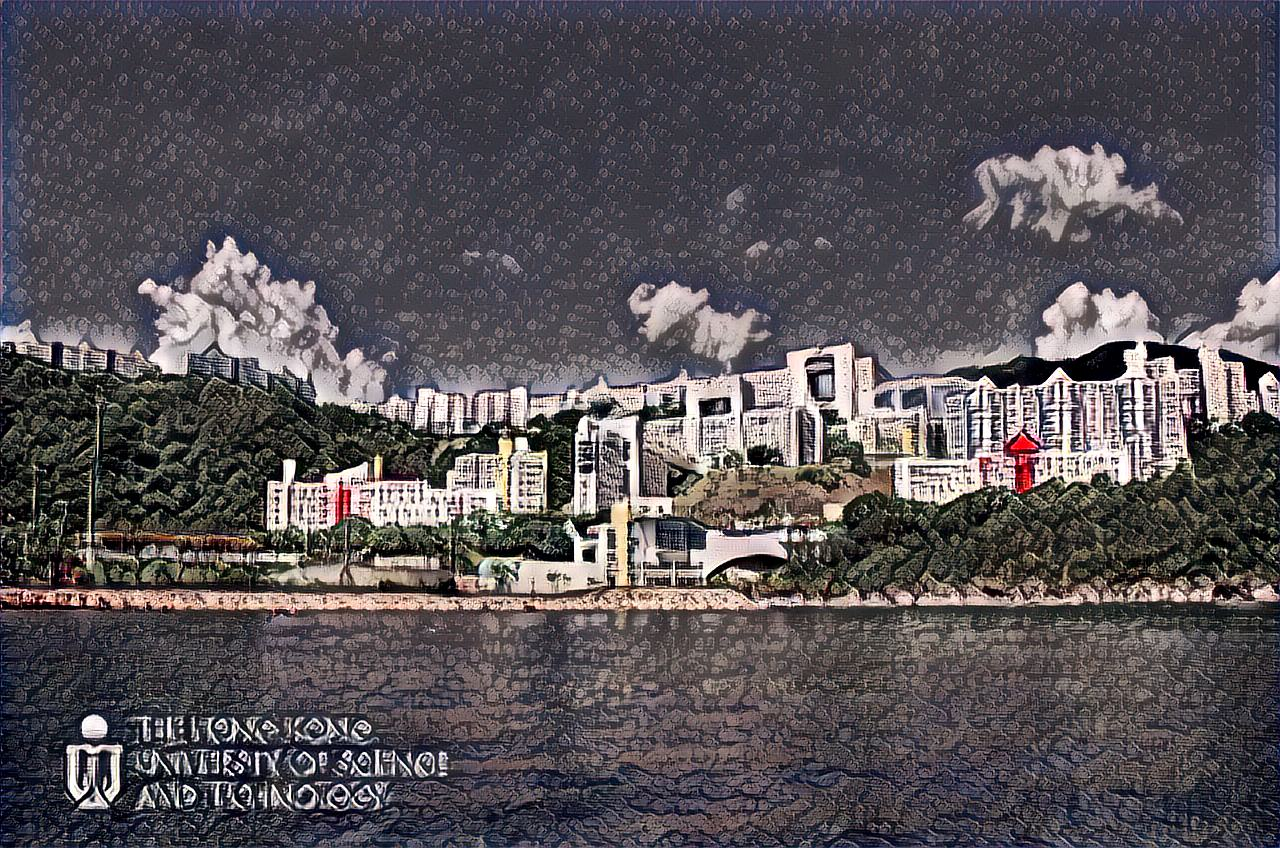
\includegraphics[width=\textwidth]{./part1_inference/output_6_boris-kustodiev_under-honey-s-harmonica-1927.jpg}
            \caption{Generated Image}
        \end{subfigure}
    \end{minipage}
    
    \vspace{0.1cm}

    \begin{minipage}{\textwidth}
        \centering
        \begin{subfigure}{0.25\textwidth}
            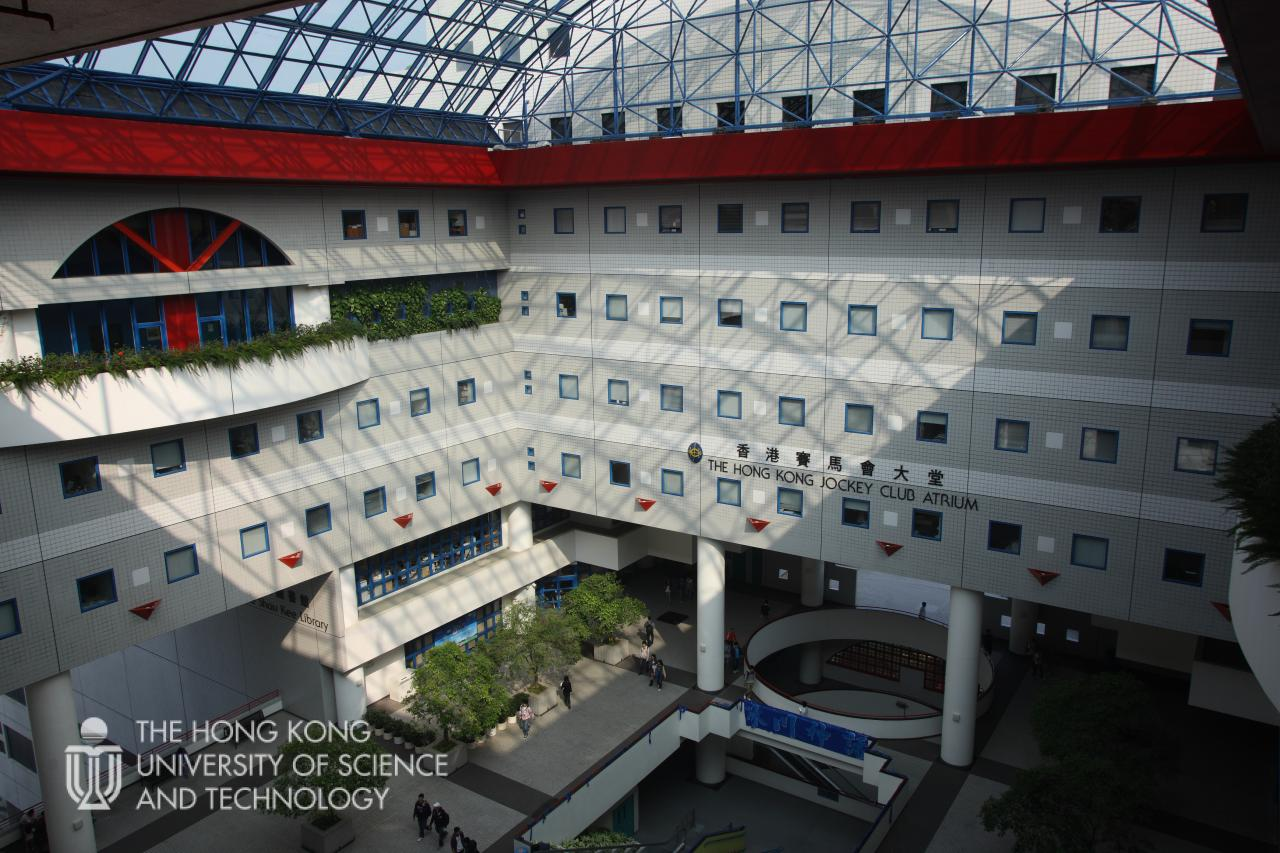
\includegraphics[width=\textwidth]{./data_set/HKUST/14.jpeg}
            \caption{Content Image}
        \end{subfigure}
        \hfill % This command adds space between the subfigures
        \begin{subfigure}{0.25\textwidth}
            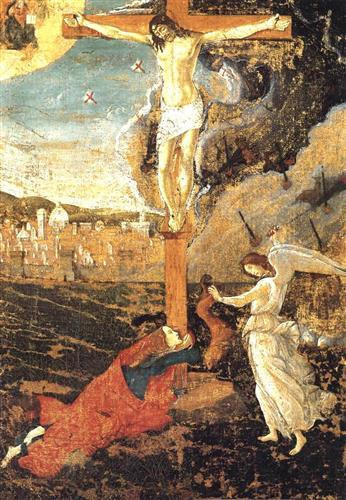
\includegraphics[width=\textwidth]{./wikiart/Early_Renaissance/sandro-botticelli_crucifixion(1).jpg}
            \caption{Style Image}
        \end{subfigure}
        \hfill % This command adds space between the subfigures
        \begin{subfigure}{0.25\textwidth}
            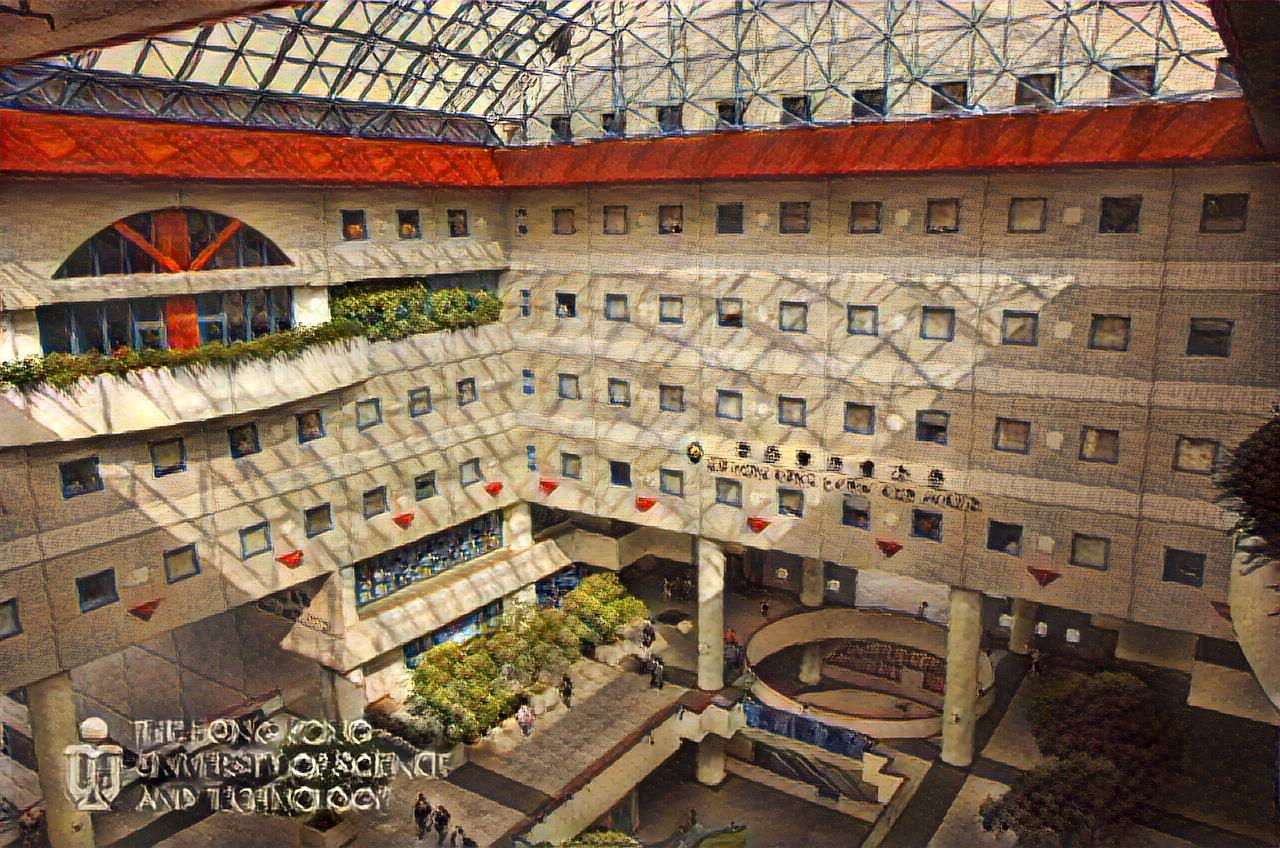
\includegraphics[width=\textwidth]{./part1_inference/output_14_sandro-botticelli_crucifixion(1).jpg}
            \caption{Generated Image}
        \end{subfigure}
    \end{minipage}    
    
    \caption{Example of Style Transfer}
    \label{fig:part1_inference}
\end{figure}



\end{document}
